\documentclass[12pt]{beamer}

\usetheme{Oxygen}
\usepackage{thumbpdf}
\usepackage{wasysym}
% \usepackage{ucs}
\usepackage[utf8]{inputenc}
\usepackage{pgf,pgfarrows,pgfnodes,pgfautomata,pgfheaps,pgfshade}
\usepackage{verbatim}
\usepackage{multicol}


\pdfinfo
{
  /Title       (Ingeniería de Software)
  /Creator     (TeX)
  /Author      (Sebastián Salazar Molina)
}


\title{Ingeniería de Software}
\subtitle{Calidad}
\author{Sebastián Salazar Molina.}
\institute[INF - UTEM] { Unidad de Informática - Universidad Tecnológica Metropolitana }
\date{27 de Abril de 2015}

\begin{document}

\frame{\titlepage}

\section*{}
\begin{frame}
  \frametitle{Contenidos}
  \begin{multicols}{2}
    \tableofcontents[section=1,hidesubsections]
  \end{multicols}
\end{frame}

\AtBeginSection[]
{
  \frame<handout:0>
  {
    \frametitle{Contenidos}
    \begin{multicols}{2}
    \tableofcontents[currentsection,hideallsubsections]
    \end{multicols}
  }
}

\AtBeginSubsection[]
{
  \frame<handout:0>
  {
    \frametitle{Contenidos}
%     \begin{multicols}{2}
    \tableofcontents[sectionstyle=show/hide,subsectionstyle=show/shaded/hide]
%     \end{multicols}
  }
}

\newcommand<>{\highlighton}[1]{%
  \alt#2{\structure{#1}}{{#1}}
}

\newcommand{\icon}[1]{\pgfimage[height=1em]{#1}}



%%%%%%%%%%%%%%%%%%%%%%%%%%%%%%%%%%%%%%%%%
%%%%%%%%%% Content starts here %%%%%%%%%%
%%%%%%%%%%%%%%%%%%%%%%%%%%%%%%%%%%%%%%%%%


% Introducción
\section{Introducción}
\subsection{Introducción}

\begin{frame}
 \begin{quote}
La calidad nunca es un accidente; siempre es el resultado de un esfuerzo de la inteligencia.
 \newline
 \raggedleft{-- John Ruskin}
 \end{quote}
\end{frame}

\subsection{La crisis del Software}
\begin{frame}
 \frametitle{El problema del Software}
Tanto la ingeniería aplicada a la fabricación de Hardware, como la ingeniería aplicada al Desarrollo de Software, han seguido caminos 
distintos, y han cosechado suertes distintas.
\newline
Mientras que la ley de Moore, se sigue cumpliendo hasta nuestros días. El campo del Software no ha cosechado la misma fortuna. 
\newline
En 1968, se dictó en la OTAN la primera conferencia sobre el desarrollo de Software, y no fue 
precisamente, por camaradería.
\end{frame}


\begin{frame}
 \frametitle{La crisis del Software}
En dicha reunión, se acuñó el termino \alert{``crisis de Software''}, que engloba una serie de críticas al desarrollo de Software:
\begin{itemize}
 \item<2-> Los proyectos no terminaban en plazo.
 \item<3-> Los proyectos no se ajustaban al presupuesto inicial.
 \item<4-> \alert{Baja calidad} del software generado.
 \item<5-> El Software no cumple con las especificaciones.
 \item<6-> El Código es inmantenible.
 \item<7-> Muchas más...
\end{itemize}
\end{frame}






\section{Definición}

\begin{frame}
\frametitle{Definición}
\begin{block}
- ``Concordancia con los requisitos funcionales y de rendimiento explícitamente establecidos con los estándares de desarrollo 
explícitamente documentados y con las características implícitas que se espera de todo software desarrollado profesionalmente''
-- R. S. Pressman
\end{block}
\end{frame}

\begin{frame}
\frametitle{Definición}
\begin{block}
- En general consideraremos un producto de calidad en la medida que este producto pueda satisfacer nuestras necesidades.
\end{block}
\end{frame}

% Calidad
\section{Calidad}
\subsection{Calidad}

\subsection{Problemas}
\begin{frame}
\frametitle{Problemas}
Aunque la definición es sencilla, cumplirla dista mucho de serlo.
\begin{itemize}
 \item<2-> Las necesidades que debe cumplir el producto de software, están dadas por las \alert{especificaciones}.
 \item<3-> La calidad del software, es medida por las \alert{expectativas} que tienen sus usuarios.
\end{itemize}
\end{frame}

\subsection{Objetivos}
\begin{frame}
\frametitle{Objetivos}
El uso de metodologías, de planificación de proyectos y de herramientas de apoyo, apuntan exclusivamente a entregar un producto de \alert{calidad}.
\end{frame}

\subsection{Técnicas comunes}
\begin{frame}
\frametitle{Métodos comunes}
Algunos grupos, consideran que dada la dificultad de asegurar la calidad del software en sí, podemos tener calidad si se definen políticas 
(las buenas prácticas), se usan estándares, y comprobamos que estos estándares sean usados en el desarrollo.
El problema es que la burocracia de estos procedimientos, generalmente entorpecen el proyecto.
\end{frame}

\subsection{Estándares}

\begin{frame}
 \frametitle{Estándares}
 Existen dos grandes categorías de Estándares
 \begin{itemize}
  \item<2-> Estándares para el Producto.
  \item<3-> Estándares para el Proceso.
 \end{itemize}
\end{frame}


\begin{frame}
 \frametitle{Estándares para el producto}
 Estándares más importantes:
 \begin{itemize}
  \item<2-> Estándar de Documentación.
  \item<3-> Estándar de Codificación.
 \end{itemize}
\end{frame}


\begin{frame}
 \frametitle{Estándares del Proceso}
 Uso de \alert{Metodologías}
 \begin{itemize}
  \item<2-> Metodología de Desarrollo (Scrum).
  \item<3-> Utilizar la herramienta adecuada.
  \item<4-> Metodología para el desarrollo del proyecto (PMBOK).
  \item<5-> Metodología para lograr Eficiencia en las Operaciones (ITIL).
 \end{itemize}
\end{frame}


\begin{frame}
 \frametitle{Atributos de Calidad}
 En la práctica, es casi imposible asegurar la calidad en un 100\%, lo usual es definir \alert{atributos} de calidad. 
 \newline
 \pause
 Los atributos, son un conjunto de características deseadas (y priorizadas), que nos comprometeremos a cumplir.
\end{frame}


\begin{frame}
 \frametitle{Atributos de Calidad}
 Ejemplo:
 \begin{itemize}
  \item<2-> Seguridad.
  \item<3-> Fiabilidad.
  \item<4-> Robustez.
  \item<5-> Usabilidad.
  \item<6-> Portabilidad.
  \item<7-> Etc...
 \end{itemize}
\end{frame}


\section{Gestión de Calidad}
\subsection{Gestión de Calidad}

\begin{frame}
\frametitle{Gestión de Calidad}
En la ISO 9000 se define la gestión de calidad como:
\pause
``El conjunto de actividades de la función general de la dirección que determina la calidad, los objetivos y las responsabilidades y se
implanta por medios tales como la planificación de la calidad, el control de la calidad, el aseguramiento (garantía) de la calidad y la
mejora de la calidad, en el marco del sistema de calidad''.
\end{frame}



\begin{frame}
\frametitle{Gestión de Calidad}
La gestión de calidad, se estructura en tres aspectos de la calidad:
\begin{itemize}
 \item<2-> Garantizarla.
 \item<3-> Planificarla.
 \item<4-> Controlarla.
\end{itemize}
\end{frame}


\begin{frame}
\frametitle{Garantía de Calidad}
La garantía de calidad, apunta a escoger los estándares más adecuados para el desarrollo del proyecto y las herramientas necesarias 
para apoyar estos estándares. Dos de las ventajas:
\begin{itemize}
 \item<2-> Se establece un marco común de trabajo.
 \item<3-> Permite la continuedad del trabajo, independiente de quienes lo desarrollan.
\end{itemize}

\end{frame}

\begin{frame}
\frametitle{Planificación de Calidad}
La planificación de la calidad, es la etapa en que se define la calidad del software (que entendemos por ``alta calidad''), las metas y 
cómo esta será \alert{medida}. 
Generalmente a través de algunos atributos deseables para el producto.
La calidad es un proceso continuo y transversal para \alert{todos} los procesos que intervienen en el desarrollo.
\end{frame}

\begin{frame}
\frametitle{Control de Calidad}
El control de calidad, es el proceso que vigila al desarrollo para asegurarse de que se cumplen tanto con los estándares como con las 
metas. En esta etapa se incluyen las mediciones.
\end{frame}

\section{Factor Humano}
\subsection{Factor Humano}

\begin{frame}
 \frametitle{Factor Humano}
 El Software es un ``producto'' construido por Humanos, y como cualquier otra cosa producida por humanos, tiene \alert{errores}.
 \newline
 \pause
 La mayoría de las veces, el software es usado por personas.
\end{frame}

\begin{frame}
 \frametitle{Puntos de Vista}
 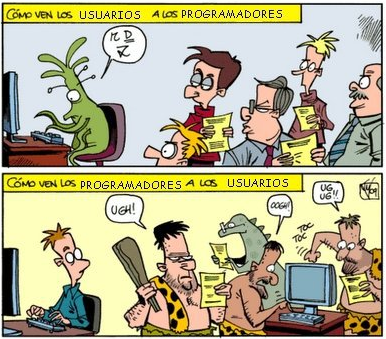
\includegraphics[scale=0.5]{img/puntos_vista.png}
\end{frame}


\begin{frame}
 \frametitle{Principal Actividad del Desarrollo de Software}
 \pause
 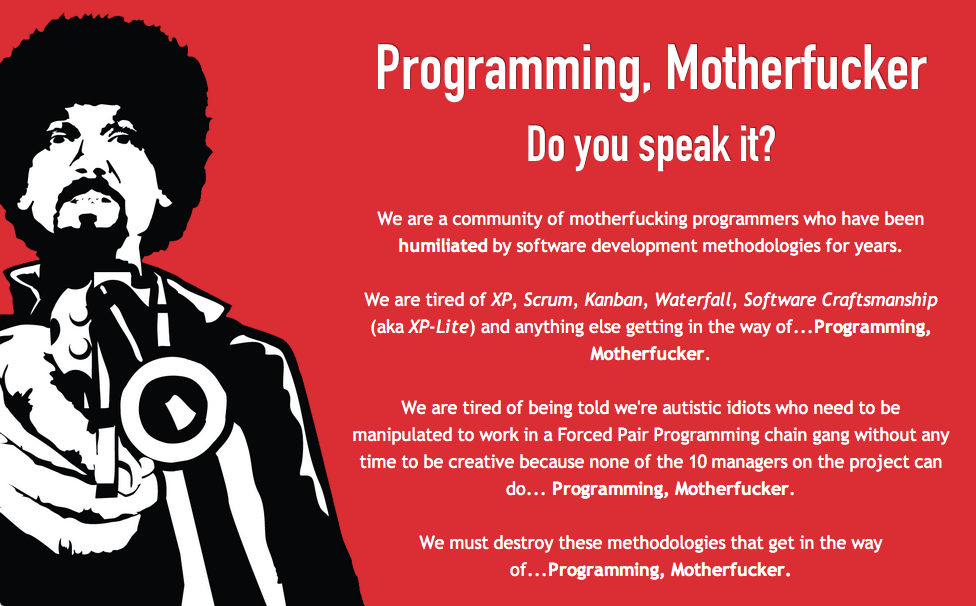
\includegraphics[scale=0.3]{img/programaCTM.png}
\end{frame}

\begin{frame}
 \frametitle{Factores Críticos}
 \begin{itemize}
  \item<2-> Motivación.
  \item<3-> Colaboración.
  \item<4-> Creatividad.
  \item<5-> Una visión común.
  \item<6-> Ser Flexibles.
 \end{itemize}
\end{frame}


\begin{frame}
 \frametitle{Factores a Evitar}
 \begin{itemize}
  \item<2-> Optimismo Forzado.
  \item<3-> Deuda Técnica.
  \item<4-> Desatender las críticas.
  \item<5-> No valorar los aportes de otras personas.
 \end{itemize}
\end{frame}



\frame{
  \vspace{2cm}
  {\huge ¿ Preguntas ?}

  \vspace{3cm}
  \begin{flushright}
    Sebastián Salazar Molina

    \structure{\footnotesize{@sebastian\_sm}}
  \end{flushright}
}

\end{document}
